% 第5章 相似矩阵及二次型（同济《线性代数》第七版 第5章）§5–§7 + 拓展（二次曲面）
% §5 二次型及其标准形；§6 用配方法化二次型成标准形；§7 正定二次型。
% 二次曲面为教材之外的拓展节（对应第8章空间解析几何相关内容），保留作几何背景。
% §1–§4 见 8.特征值&特征向量&相似矩阵.tex。正文不写例题与习题。

\section{二次型及其标准形}

\subsection{二次型及其矩阵}
\begin{definition}[二次型]
含有$n$个变量$x_1,x_2,\dots,x_n$的二次齐次函数
\[
\begin{aligned}
f(x_1,x_2,\dots,x_n)={}&a_{11}x_1^{2}+a_{22}x_2^{2}+\dots+a_{nn}x_n^{2}\\
&+2a_{12}x_1x_2+2a_{13}x_1x_3+\dots+2a_{n-1,n}x_{n-1}x_n
\end{aligned}
\]
称为\textbf{二次型}。当系数$a_{ij}$全为实数时称为\textbf{实二次型}，含有复数系数时称为复二次型。本书只讨论实二次型。
\end{definition}

取$a_{ij}=a_{ji}$（$i<j$），则$2a_{ij}x_ix_j=a_{ij}x_ix_j+a_{ji}x_jx_i$，于是
\[
f=\sum_{i=1}^{n}\sum_{j=1}^{n}a_{ij}x_ix_j .
\]
记$\boldsymbol{x}=(x_1,x_2,\dots,x_n)^{T}$，
\[
A=\begin{pmatrix}
a_{11}&a_{12}&\dots&a_{1n}\\
a_{21}&a_{22}&\dots&a_{2n}\\
\vdots&\vdots&\ddots&\vdots\\
a_{n1}&a_{n2}&\dots&a_{nn}
\end{pmatrix}
\quad(a_{ij}=a_{ji}),
\]
则二次型可用矩阵记号写成
\[
f=\boldsymbol{x}^{T}A\boldsymbol{x},
\]
其中$A$为\textbf{对称矩阵}，称为二次型$f$的\textbf{矩阵}；$A$的秩称为二次型$f$的\textbf{秩}。

任给一个二次型，就唯一确定一个对称矩阵；任给一个对称矩阵，也可唯一确定一个二次型。因此二次型与对称矩阵之间存在\textbf{一一对应}关系，对称矩阵$A$也叫做二次型$f$的矩阵，$f$叫做对称矩阵$A$的二次型。

只含平方项的二次型称为\textbf{标准形}；形如
\[
f=y_1^{2}+\dots+y_p^{2}-y_{p+1}^{2}-\dots-y_{p+q}^{2}
\]
的标准形称为\textbf{规范形}。

\subsection{合同矩阵}
我们讨论的主要问题是：是否存在可逆线性变换$\boldsymbol{x}=C\boldsymbol{y}$（若存在，如何寻找），使二次型化为标准形。把$\boldsymbol{x}=C\boldsymbol{y}$代入$f=\boldsymbol{x}^{T}A\boldsymbol{x}$，得
\[
f=\boldsymbol{x}^{T}A\boldsymbol{x}=(C\boldsymbol{y})^{T}A(C\boldsymbol{y})
=\boldsymbol{y}^{T}(C^{T}AC)\boldsymbol{y}.
\]
记$B=C^{T}AC$，则$B$仍为对称矩阵，且$R(B)=R(A)$（$C$可逆），$B$就是变换后二次型的矩阵。

\begin{definition}[合同]
设$A$和$B$是$n$阶矩阵，若有可逆矩阵$C$，使
\[
B=C^{T}AC,
\]
则称矩阵$A$与$B$\textbf{合同}。
\end{definition}

合同关系具有自反性、对称性、传递性。若$A$为对称矩阵，则$B=C^{T}AC$也是对称矩阵，且$R(B)=R(A)$——即\textbf{经可逆线性变换，二次型的矩阵变为与之合同的矩阵，二次型的秩不变}。

于是"用可逆线性变换化二次型为标准形"等价于"求可逆矩阵$C$使$C^{T}AC$为对角矩阵"，这个问题称为把对称矩阵$A$\textbf{合同对角化}。

\subsection{用正交变换化二次型为标准形}
\begin{theorem}[正交变换化标准形]
任给二次型$f=\sum_{i,j=1}^{n}a_{ij}x_ix_j=\boldsymbol{x}^{T}A\boldsymbol{x}$（$A^{T}=A$），总有\textbf{正交变换}$\boldsymbol{x}=P\boldsymbol{y}$，使$f$化为标准形
\[
f=\lambda_1y_1^{2}+\lambda_2y_2^{2}+\dots+\lambda_ny_n^{2},
\]
其中$\lambda_1,\lambda_2,\dots,\lambda_n$是$A$的$n$个特征值。
\end{theorem}

这是因为实对称矩阵$A$必有正交矩阵$P$使$P^{-1}AP=P^{T}AP=\Lambda$（第4节定理），令$\boldsymbol{x}=P\boldsymbol{y}$即得。此时$P$的列向量是$A$的$n$个两两正交的单位特征向量。

\begin{corollary}
任给$n$元二次型$f=\boldsymbol{x}^{T}A\boldsymbol{x}$，总有可逆变换$\boldsymbol{x}=C\boldsymbol{z}$，使$f(C\boldsymbol{z})$为规范形。
\end{corollary}

证明思路：先由定理取正交变换化为$\lambda_1y_1^{2}+\dots+\lambda_ny_n^{2}$，设$f$的秩为$r$，则恰有$r$个$\lambda_i\ne0$；再令$y_i=\dfrac{z_i}{\sqrt{|\lambda_i|}}$（$i\le r$），$y_i=z_i$（$i>r$），即得系数为$\pm1$或$0$的规范形。

\subsubsection{正交变换法的步骤}
\begin{enumerate}
    \item 写出二次型的矩阵$A$（注意：交叉项$x_ix_j$的系数要\textbf{平分}到$a_{ij}$与$a_{ji}$两处）。
    \item 求$A$的特征值$\lambda_1,\dots,\lambda_n$及对应的两两正交的单位特征向量$\boldsymbol{p}_1,\dots,\boldsymbol{p}_n$（同一重特征值处需施密特正交化）。
    \item 令$P=(\boldsymbol{p}_1,\dots,\boldsymbol{p}_n)$，作正交变换$\boldsymbol{x}=P\boldsymbol{y}$，则
    \[
    f=\lambda_1y_1^{2}+\lambda_2y_2^{2}+\dots+\lambda_ny_n^{2}.
    \]
\end{enumerate}

正交变换的优点是保持几何形状不变（保长度、保内积），因此常用于判断二次曲面/二次曲线的类型。

\subsection*{附：用初等变换（合同变换）化标准形}
配方法用矩阵语言表达，就是对$A$作一列"协调一致"的初等行、列变换（$C^{T}AC$）。把单位矩阵放在$A$下面构成$2n\times n$矩阵$\begin{pmatrix}A\\E\end{pmatrix}$，每对$A$作一次列变换，就同时对$A$作一次相应的行变换（左乘、右乘同一个初等矩阵的转置），即
\[
\begin{pmatrix}A\\E\end{pmatrix}\longrightarrow\begin{pmatrix}C^{T}AC\\C\end{pmatrix}.
\]
当$C^{T}AC$化为对角矩阵时，下面的$E$就化成了所求的合同变换矩阵$C$。这就是\textbf{初等变换法}（也叫合同变换法），与配方法等价。

\keyformula{f=\boldsymbol{x}^{T}A\boldsymbol{x}\ (A^{T}=A),\qquad \boldsymbol{x}=C\boldsymbol{y}\ \Rightarrow\ f=\boldsymbol{y}^{T}(C^{T}AC)\boldsymbol{y},\qquad B=C^{T}AC\iff A\ \text{与}\ B\ \text{合同}}

\keyformula{\boldsymbol{x}=P\boldsymbol{y}\ (P^{T}P=E)\ \Rightarrow\ f=\lambda_1y_1^{2}+\dots+\lambda_ny_n^{2},\quad \lambda_i\ \text{为}\ A\ \text{的特征值}}

\corepoint{
（1）写矩阵时交叉项系数必须\textbf{除以2}：$f=2x_1x_2$对应$a_{12}=a_{21}=1$。这是二次型部分最高频的错误。\\
（2）正交变换得到的标准形系数\textbf{恰是特征值}，且系数顺序与$P$中列向量顺序一致；配方法得到的标准形系数则与所用变换有关，不唯一。\\
（3）正交变换化标准形\textbf{不改变}二次型的秩与正、负惯性指数；配方法同样不改变。\\
（4）正交变换下$C^{T}AC=C^{-1}AC$（因为$C^{T}=C^{-1}$），所以"合同"与"相似"在正交变换这一特殊情形下重合；一般情形两者不同。
}

\section{用配方法化二次型成标准形}

用正交变换化标准形需要求特征值、解特征向量，计算量大；若只要求"用可逆线性变换化标准形"，用拉格朗日配方法更简便，只是所得标准形不唯一。

\subsection{配方法的两种情形}
\textbf{情形一：二次型中含有某个变量的平方项。}\quad 不妨设含$x_1^{2}$，把含有$x_1$的所有项集中起来配成完全平方，剩下的是不含$x_1$的$n-1$元二次型，再对它重复上述步骤。具体地，若
\[
f=a_{11}x_1^{2}+2a_{12}x_1x_2+\dots+2a_{1n}x_1x_n+g(x_2,\dots,x_n),
\]
则
\[
f=\frac{1}{a_{11}}\bigl(a_{11}x_1+a_{12}x_2+\dots+a_{1n}x_n\bigr)^{2}
+g_1(x_2,\dots,x_n),
\]
其中$g_1$仍是二次型。令
\[
y_1=a_{11}x_1+a_{12}x_2+\dots+a_{1n}x_n,\quad y_i=x_i\ (i\ge2),
\]
这是可逆线性变换（系数矩阵为上三角且对角元非零），在此变换下$f$化为只含$y_2,\dots,y_n$的二次型，继续配方即可。

\textbf{情形二：二次型中不含任何平方项。}\quad 此时必有某个交叉项，例如$2a_{12}x_1x_2$（$a_{12}\ne0$）。先作可逆变换
\[
\begin{cases}
x_1=y_1+y_2,\\
x_2=y_1-y_2,\\
x_i=y_i\quad(i\ge3),
\end{cases}
\]
则$2a_{12}x_1x_2=2a_{12}(y_1^{2}-y_2^{2})$，出现了平方项，就化为情形一，继续配方。

\subsection{配方法的步骤}
\begin{enumerate}
    \item 若含平方项，就按上面的公式对第一个平方项变量配方，把含它的项全部吸收进完全平方，得到一个新的二次型（变量少一个）。
    \item 若不含平方项，先用$x_1=y_1+y_2,\ x_2=y_1-y_2$造出平方项。
    \item 重复以上两步，直到只剩平方项，得标准形$f=k_1z_1^{2}+\dots+k_rz_r^{2}$。
    \item 把各步的变换\textbf{复合}（依次代入），写出总的可逆线性变换$\boldsymbol{x}=C\boldsymbol{z}$及变换矩阵$C$。复合时注意"先作的变换在右边"。
\end{enumerate}

\corepoint{
（1）配方时必须把\textbf{所有}含该变量的项（包括交叉项）一次吸收干净，否则后面无法继续。\\
（2）情形二中若同时有多个交叉项，只需挑一个造平方项即可，不必全处理。\\
（3）最后求变换矩阵时，要把分步变换依次代入合成一个矩阵，不能只写最后一步的矩阵。\\
（4）标准形中系数为$0$的项可以省略，但写变换矩阵时对应的变量仍要保留（否则矩阵不满秩，不是可逆变换）。\\
（5）配方法不改变二次型的秩与惯性指数，可用这一点验算。
}

\keyformula{a_{11}x_1^{2}+2\sum_{j\ge2}a_{1j}x_1x_j=\frac{1}{a_{11}}\Bigl(\sum_{j\ge1}a_{1j}x_j\Bigr)^{2}-\frac{1}{a_{11}}\Bigl(\sum_{j\ge2}a_{1j}x_j\Bigr)^{2}}

\keyformula{x_1=y_1+y_2,\ x_2=y_1-y_2\ \Rightarrow\ 2a_{12}x_1x_2=2a_{12}y_1^{2}-2a_{12}y_2^{2}}

\keyformula{f\ \xrightarrow{\ \boldsymbol{x}=C\boldsymbol{y}\ }\ k_1y_1^{2}+\dots+k_ny_n^{2}\qquad(C\ \text{可逆})}

\section{正定二次型}

\subsection{惯性定理}
二次型的标准形显然不唯一，但标准形中所含\textbf{项数}（即二次型的秩）是确定的。不仅如此，在限定变换为实变换时，标准形中\textbf{正系数的个数}也是不变的：

\begin{theorem}[惯性定理]
设二次型$f=\boldsymbol{x}^{T}A\boldsymbol{x}$的秩为$r$，且有两个可逆变换$\boldsymbol{x}=C_1\boldsymbol{y}$及$\boldsymbol{x}=C_2\boldsymbol{z}$使
\[
f=k_1y_1^{2}+\dots+k_ry_r^{2}\quad(k_i\ne0),
\qquad
f=l_1z_1^{2}+\dots+l_rz_r^{2}\quad(l_i\ne0),
\]
则$k_1,\dots,k_r$中正数的个数与$l_1,\dots,l_r$中正数的个数相等（从而负数的个数也相等）。
\end{theorem}

二次型的标准形中正系数的个数称为二次型的\textbf{正惯性指数}，负系数的个数称为\textbf{负惯性指数}。若正惯性指数为$p$、秩为$r$，则负惯性指数为$r-p$，且$f$的\textbf{规范形}唯一确定：
\[
f=z_1^{2}+\dots+z_p^{2}-z_{p+1}^{2}-\dots-z_r^{2}.
\]

因此，两个$n$元实二次型合同$\iff$它们有相同的秩与相同的正惯性指数。

\subsection{正定二次型与正定矩阵}
\begin{definition}[正定、负定]
设二次型$f=\boldsymbol{x}^{T}A\boldsymbol{x}$，若对任何$\boldsymbol{x}\ne\boldsymbol{0}$都有$f(\boldsymbol{x})>0$（显然$f(\boldsymbol{0})=0$），则称$f$为\textbf{正定二次型}，并称对称矩阵$A$是\textbf{正定}的；若对任何$\boldsymbol{x}\ne\boldsymbol{0}$都有$f(\boldsymbol{x})<0$，则称$f$为\textbf{负定二次型}，并称$A$是\textbf{负定}的。
\end{definition}

\begin{theorem}[正定的标准形判据]
$n$元二次型$f=\boldsymbol{x}^{T}A\boldsymbol{x}$为正定的充分必要条件是：它的标准形的$n$个系数全为正，即它的规范形的$n$个系数全为$1$，亦即它的\textbf{正惯性指数等于$n$}。
\end{theorem}

\textbf{证明}\quad 设可逆变换$\boldsymbol{x}=C\boldsymbol{y}$使$f=\sum k_iy_i^{2}$。充分性：若$k_i>0$，则对$\boldsymbol{x}\ne\boldsymbol{0}$有$\boldsymbol{y}=C^{-1}\boldsymbol{x}\ne\boldsymbol{0}$，故$f=\sum k_iy_i^{2}>0$。必要性：反证，若某个$k_i\le0$，取$\boldsymbol{y}=\boldsymbol{e}_i$（单位坐标向量），则$\boldsymbol{x}=C\boldsymbol{e}_i\ne\boldsymbol{0}$而$f(\boldsymbol{e}_i)=k_i\le0$，与正定矛盾。\hfill$\square$

\begin{corollary}[特征值判据]
对称矩阵$A$为正定的充分必要条件是$A$的特征值全为正。
\end{corollary}

\begin{corollary}[$A=Q^{T}Q$判据]
实二次型$f=\boldsymbol{x}^{T}A\boldsymbol{x}$为正定的充分必要条件是：存在可逆矩阵$Q$，使
\[
A=Q^{T}Q .
\]
\end{corollary}

\begin{theorem}[顺序主子式判据，Hurwitz]
对称矩阵$A$为正定的充分必要条件是：$A$的\textbf{各阶顺序主子式全为正}，即
\[
a_{11}>0,\qquad
\begin{vmatrix}a_{11}&a_{12}\\a_{21}&a_{22}\end{vmatrix}>0,\qquad\dots,\qquad
\begin{vmatrix}
a_{11}&a_{12}&\dots&a_{1n}\\
a_{21}&a_{22}&\dots&a_{2n}\\
\vdots&\vdots&&\vdots\\
a_{n1}&a_{n2}&\dots&a_{nn}
\end{vmatrix}>0 .
\]
对称矩阵$A$为负定的充分必要条件是：\textbf{奇数阶顺序主子式为负，偶数阶顺序主子式为正}。
\end{theorem}

这里"$k$阶顺序主子式"指$A$的前$k$行、前$k$列构成的$k$阶子式。

\subsection{正定性的判定步骤}
\begin{enumerate}
    \item 写出二次型的对称矩阵$A$。
    \item 首选\textbf{顺序主子式}：计算$\Delta_1,\Delta_2,\dots,\Delta_n$。全正$\Rightarrow$正定；奇数阶为负、偶数阶为正$\Rightarrow$负定。
    \item 若只需判断"是否正定"而矩阵阶数较大，可先用特征值或配方法求出正惯性指数，看是否为$n$。
    \item 含参数的问题：令$\Delta_k>0$（或负定条件）解出参数范围。
\end{enumerate}

\corepoint{
（1）顺序主子式必须\textbf{从左上角依次取}，不能取任意主子式；只验$|A|>0$不能推出正定（如$\operatorname{diag}(-1,-1)$）。\\
（2）正定$\Rightarrow$$|A|>0$；但$|A|>0$不一定正定，也不一定是负定判据。\\
（3）负定的判据符号是"奇负偶正"，与正定"全正"别混。\\
（4）只有\textbf{实对称矩阵}才谈正定；非对称矩阵即使$x^{T}Ax>0$恒成立，通常也先对称化再讨论。\\
（5）几何意义：二元正定二次型$f(x,y)=c\ (c>0)$是一族以原点为中心的椭圆；三元正定二次型$f(x,y,z)=c\ (c>0)$是一族椭球面——这是正定性最直观的图景。
}

\keyformula{f\ \text{正定}\iff p=n\iff \lambda_i>0\ (\forall i)\iff \Delta_k>0\ (k=1,\dots,n)\iff \exists\,Q\ \text{可逆},\ A=Q^{T}Q}

\keyformula{f\ \text{负定}\iff (-1)^{k}\Delta_k>0\ (k=1,\dots,n),\qquad \text{规范形：}\ z_1^{2}+\dots+z_p^{2}-z_{p+1}^{2}-\dots-z_r^{2}}

\section{拓展：空间中的曲面与二次曲面}

本节是教材之外的几何拓展，把第5节的二次型理论落到三维空间，用于识别三元二次方程所表示的曲面。

\subsection{曲面方程与几类特殊曲面}
给定空间直角坐标系，若曲面$S$上点的坐标都满足方程$F(x,y,z)=0$，且坐标满足该方程的点都在$S$上，则称$F(x,y,z)=0$为曲面$S$的\textbf{方程}，$S$为该方程的\textbf{图形}。

\textbf{球面}\quad 球心$M_0(x_0,y_0,z_0)$、半径$r$的球面方程为
\[
(x-x_0)^{2}+(y-y_0)^{2}+(z-z_0)^{2}=r^{2},
\]
展开后是三元二次方程，其特点是：$x^{2},y^{2},z^{2}$的系数相同且没有$xy,yz,zx$项。具有这三个条件的方程，配方后若右端$k>0$为球面，$k=0$为一点（点球面），$k<0$无图形（虚球面）。

\textbf{柱面}\quad 平行于定直线并沿定曲线$C$移动的直线$L$形成的轨迹叫做\textbf{柱面}，$C$叫\textbf{准线}，$L$叫\textbf{母线}。只含两个变量的方程在空间中表示柱面，其母线平行于方程中不出现的那个变量所对应的坐标轴。例如$\dfrac{x^{2}}{a^{2}}+\dfrac{y^{2}}{b^{2}}=1$、$\dfrac{x^{2}}{a^{2}}-\dfrac{y^{2}}{b^{2}}=1$、$x^{2}=2py$分别表示母线平行于$z$轴的椭圆柱面、双曲柱面、抛物柱面。

\textbf{旋转曲面}\quad 由一条平面曲线$C$绕该平面上的一条定直线$L$旋转一周所成的曲面叫做\textbf{旋转曲面}，$C$叫母线，$L$叫旋转轴。位于$yOz$面上的曲线$f(y,z)=0$绕$z$轴旋转所得曲面方程为
\[
f\bigl(\pm\sqrt{x^{2}+y^{2}},\ z\bigr)=0 ;
\]
绕$y$轴旋转则为$f\bigl(y,\pm\sqrt{x^{2}+z^{2}}\bigr)=0$。口诀：\textbf{与旋转轴同名的变量不动，另一变量换成另两个变量平方和的平方根}。

\textbf{空间曲线}\quad 空间曲线可看作两个曲面的交线，其一般方程为
\[
\begin{cases}F(x,y,z)=0,\\ G(x,y,z)=0,\end{cases}
\]
也可写成参数方程$x=x(t),\ y=y(t),\ z=z(t)$。以$C$为准线、母线垂直于平面$\pi$的柱面与$\pi$的交线叫做$C$在$\pi$上的\textbf{投影}；从$C$的方程中消去$z$得柱面方程$F(x,y)=0$，则$\begin{cases}F(x,y)=0\\ z=0\end{cases}$就是$C$在$xOy$面上的投影曲线。

\subsection{二次曲面的类型}
一般的三元二次方程可写成
\[
\boldsymbol{x}^{T}A\boldsymbol{x}+\boldsymbol{v}^{T}\boldsymbol{x}+a_{44}=0,
\qquad
A=(a_{ij})_{3\times3}\ (a_{ij}=a_{ji}),\ \boldsymbol{x}=(x,y,z)^{T},\ \boldsymbol{v}=(a_{14},a_{24},a_{34})^{T}.
\]
由第5节的正交变换定理，存在正交变换$\boldsymbol{x}=P\boldsymbol{y}$把二次型$\boldsymbol{x}^{T}A\boldsymbol{x}$化为$\lambda_1x'^{2}+\lambda_2y'^{2}+\lambda_3z'^{2}$，即存在适当的直角坐标系使原方程化为
\[
\lambda_1x'^{2}+\lambda_2y'^{2}+\lambda_3z'^{2}+a'_{14}x'+a'_{24}y'+a'_{34}z'+a'_{44}=0 .
\]
对系数的各种情况分类讨论，即得下列九类二次曲面：

\begin{table}[htbp]
\centering
\caption{九类二次曲面的标准方程}
\begin{adjustbox}{max width=\linewidth}
\begin{tabular}{@{}lll@{}}
\toprule
名称 & 标准方程 & 方程特点\\
\midrule
椭圆柱面 & $\dfrac{x^{2}}{a^{2}}+\dfrac{y^{2}}{b^{2}}=1$ & 缺一个变量，母线平行于该轴\\
双曲柱面 & $\dfrac{x^{2}}{a^{2}}-\dfrac{y^{2}}{b^{2}}=1$ & 缺一个变量，两平方项异号\\
抛物柱面 & $x^{2}=2py\ (p>0)$ & 缺一个变量，含一次项\\
椭球面 & $\dfrac{x^{2}}{a^{2}}+\dfrac{y^{2}}{b^{2}}+\dfrac{z^{2}}{c^{2}}=1$ & 三个平方项系数同号\\
单叶双曲面 & $\dfrac{x^{2}}{a^{2}}+\dfrac{y^{2}}{b^{2}}-\dfrac{z^{2}}{c^{2}}=1$ & 两正一负，常数项为$1$\\
双叶双曲面 & $\dfrac{x^{2}}{a^{2}}-\dfrac{y^{2}}{b^{2}}-\dfrac{z^{2}}{c^{2}}=1$ & 一正两负，常数项为$1$\\
椭圆抛物面 & $\dfrac{x^{2}}{2p}+\dfrac{y^{2}}{2q}=z\ (p,q\ \text{同号})$ & 两平方项同号，一次项\\
双曲抛物面 & $\dfrac{x^{2}}{2p}-\dfrac{y^{2}}{2q}=z\ (p,q\ \text{同号})$ & 两平方项异号，一次项\\
二次锥面 & $\dfrac{x^{2}}{a^{2}}+\dfrac{y^{2}}{b^{2}}-\dfrac{z^{2}}{c^{2}}=0$ & 二次齐次，常数项为$0$\\
\bottomrule
\end{tabular}
\end{adjustbox}
\end{table}

\textbf{椭球面}\quad $\dfrac{x^{2}}{a^{2}}+\dfrac{y^{2}}{b^{2}}+\dfrac{z^{2}}{c^{2}}=1$（$a,b,c>0$），$a,b,c$称为三个半轴。$a=b=c$时为球面；有两个相等时为旋转椭球面。图形关于三个坐标面、三个坐标轴及原点都对称，且被限制在长方体$|x|\le a,\ |y|\le b,\ |z|\le c$内。用$z=h$（$|h|<c$）截割，截线是椭圆
\[
\Bigl(\frac{x}{a\sqrt{1-h^{2}/c^{2}}}\Bigr)^{2}+\Bigl(\frac{y}{b\sqrt{1-h^{2}/c^{2}}}\Bigr)^{2}=1,
\]
随$|h|\to c$椭圆缩成点$(0,0,\pm c)$。

\textbf{单叶双曲面}\quad $\dfrac{x^{2}}{a^{2}}+\dfrac{y^{2}}{b^{2}}-\dfrac{z^{2}}{c^{2}}=1$。用$z=h$截得椭圆，半轴随$|h|$增大而增大；用$y=k$截得双曲线，$|k|<b$时实轴平行于$x$轴，$|k|>b$时实轴平行于$z$轴，$|k|=b$时截线退化为两条相交直线。

\textbf{双叶双曲面}\quad $\dfrac{x^{2}}{a^{2}}-\dfrac{y^{2}}{b^{2}}-\dfrac{z^{2}}{c^{2}}=1$。用$z=h$或$y=h$截得双曲线；用$x=h$（$|h|\ge a$）截得椭圆。

\textbf{椭圆抛物面}\quad $\dfrac{x^{2}}{2p}+\dfrac{y^{2}}{2q}=z$（$p,q$同号）。用$z=h$（$h$与$p,q$同号）截得椭圆；用$x=h$或$y=h$截得抛物线。

\textbf{双曲抛物面（马鞍面）}\quad $\dfrac{x^{2}}{2p}-\dfrac{y^{2}}{2q}=z$（$p,q$同号）。用$z=h\ne0$截得双曲线（$h$与$p,q$同号时实轴平行于$x$轴，异号时平行于$y$轴）；用$z=0$截得两条相交直线；用$x=h$或$y=h$截得抛物线。

\textbf{二次锥面}\quad $\dfrac{x^{2}}{a^{2}}+\dfrac{y^{2}}{b^{2}}-\dfrac{z^{2}}{c^{2}}=0$。是二次齐次方程，若$M_0(x_0,y_0,z_0)$在锥面上，则整条过原点与$M_0$的直线都在锥面上（锥面的"直纹"性质）；用$z=h\ne0$截得椭圆，与$z=0$只交于原点。$a=b$时为圆锥面。

\begin{figure}[htbp]
\centering
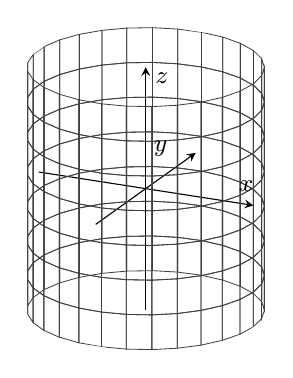
\begin{tikzpicture}
\begin{axis}[width=0.46\textwidth,height=6cm,view={25}{18},axis lines=center,ticks=none,
  xlabel=$x$,ylabel=$y$,zlabel=$z$,label style={font=\small}]
\addplot3[mesh,draw=black!75,line width=0.3pt,domain=0:360,y domain=-1.6:1.6,samples=30,samples y=8]
({1.0*cos(x)},{0.75*sin(x)},{y});
\end{axis}
\end{tikzpicture}\hfill
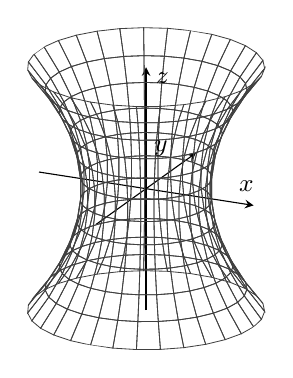
\begin{tikzpicture}
\begin{axis}[width=0.46\textwidth,height=6cm,view={25}{18},axis lines=center,ticks=none,
  xlabel=$x$,ylabel=$y$,zlabel=$z$,label style={font=\small}]
\addplot3[mesh,draw=black!75,line width=0.3pt,domain=0:360,y domain=-1.5:1.5,samples=32,samples y=12]
({(0.55+0.20*y^2)*cos(x)},{(0.55+0.20*y^2)*sin(x)},{y});
\end{axis}
\end{tikzpicture}
\caption{左：柱面（母线平行于$z$轴，准线为$xOy$面上的曲线）\quad 右：旋转曲面（$yOz$面上曲线绕$z$轴旋转，$f(\pm\sqrt{x^2+y^2},z)=0$）}
\end{figure}

\begin{figure}[htbp]
\centering
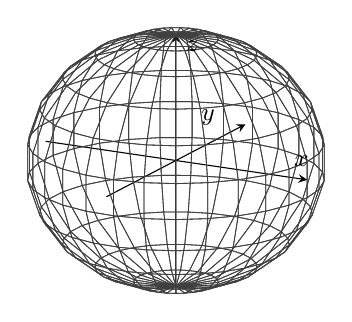
\begin{tikzpicture}
\begin{axis}[width=0.55\textwidth,height=6.2cm,view={28}{18},axis lines=center,ticks=none,
  xlabel=$x$,ylabel=$y$,zlabel=$z$,label style={font=\small}]
\addplot3[mesh,draw=black!75,line width=0.3pt,domain=0:360,y domain=0:180,samples=30,samples y=12]
({1.6*sin(y)*cos(x)},{1.1*sin(y)*sin(x)},{1.2*cos(y)});
\end{axis}
\end{tikzpicture}
\caption{椭球面$\dfrac{x^{2}}{a^{2}}+\dfrac{y^{2}}{b^{2}}+\dfrac{z^{2}}{c^{2}}=1$}
\end{figure}

\begin{figure}[htbp]
\centering
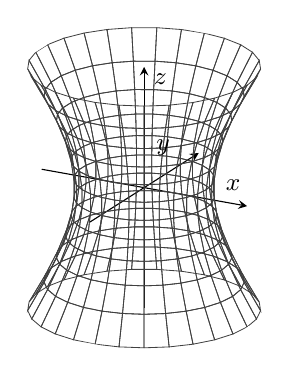
\begin{tikzpicture}
\begin{axis}[width=0.46\textwidth,height=6cm,view={28}{18},axis lines=center,ticks=none,
  xlabel=$x$,ylabel=$y$,zlabel=$z$,label style={font=\small}]
\addplot3[mesh,draw=black!75,line width=0.3pt,domain=0:360,y domain=-1.1:1.1,samples=30,samples y=12]
({1.3*cosh(y)*cos(x)},{1.0*cosh(y)*sin(x)},{0.9*sinh(y)});
\end{axis}
\end{tikzpicture}\hfill
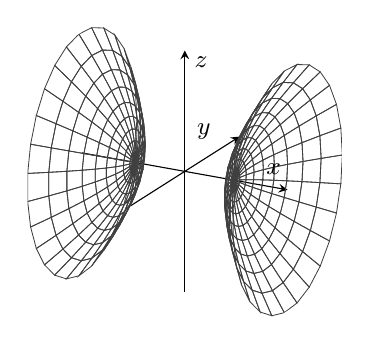
\begin{tikzpicture}
\begin{axis}[width=0.46\textwidth,height=6cm,view={28}{18},axis lines=center,ticks=none,
  xlabel=$x$,ylabel=$y$,zlabel=$z$,label style={font=\small}]
\addplot3[mesh,draw=black!75,line width=0.3pt,domain=0:360,y domain=0:1.35,samples=28,samples y=10]
({1.3*cosh(y)},{0.9*sinh(y)*cos(x)},{1.0*sinh(y)*sin(x)});
\addplot3[mesh,draw=black!75,line width=0.3pt,domain=0:360,y domain=0:1.35,samples=28,samples y=10]
({-1.3*cosh(y)},{0.9*sinh(y)*cos(x)},{1.0*sinh(y)*sin(x)});
\end{axis}
\end{tikzpicture}
\caption{左：单叶双曲面$\dfrac{x^{2}}{a^{2}}+\dfrac{y^{2}}{b^{2}}-\dfrac{z^{2}}{c^{2}}=1$\quad 右：双叶双曲面$\dfrac{x^{2}}{a^{2}}-\dfrac{y^{2}}{b^{2}}-\dfrac{z^{2}}{c^{2}}=1$}
\end{figure}

\begin{figure}[htbp]
\centering
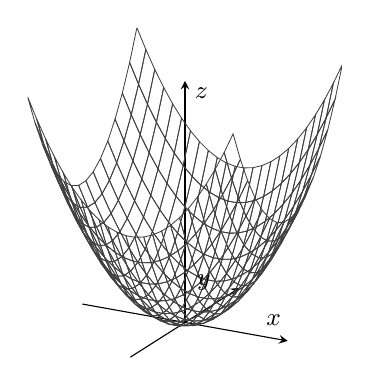
\begin{tikzpicture}
\begin{axis}[width=0.46\textwidth,height=6cm,view={28}{18},axis lines=center,ticks=none,
  xlabel=$x$,ylabel=$y$,zlabel=$z$,label style={font=\small}]
\addplot3[mesh,draw=black!75,line width=0.3pt,samples=24,domain=-1.2:1.2,y domain=-1.2:1.2,samples y=16]
{x^2+y^2};
\end{axis}
\end{tikzpicture}\hfill
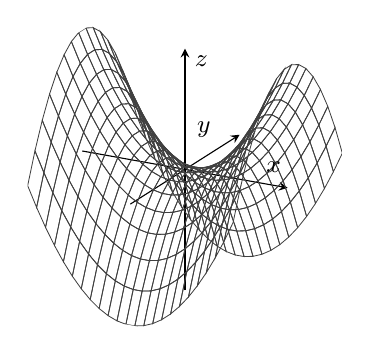
\begin{tikzpicture}
\begin{axis}[width=0.46\textwidth,height=6cm,view={28}{18},axis lines=center,ticks=none,
  xlabel=$x$,ylabel=$y$,zlabel=$z$,label style={font=\small}]
\addplot3[mesh,draw=black!75,line width=0.3pt,samples=24,domain=-1.2:1.2,y domain=-1.2:1.2,samples y=16]
{x^2-y^2};
\end{axis}
\end{tikzpicture}
\caption{左：椭圆抛物面$\dfrac{x^{2}}{2p}+\dfrac{y^{2}}{2q}=z$\quad 右：双曲抛物面（马鞍面）$\dfrac{x^{2}}{2p}-\dfrac{y^{2}}{2q}=z$}
\end{figure}

\begin{figure}[htbp]
\centering
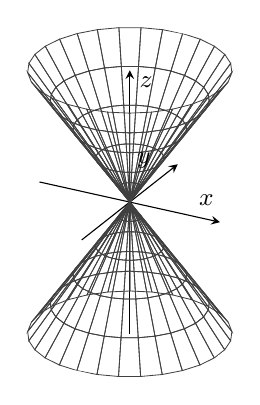
\begin{tikzpicture}
\begin{axis}[width=0.42\textwidth,height=6.4cm,view={28}{18},axis lines=center,ticks=none,
  xlabel=$x$,ylabel=$y$,zlabel=$z$,label style={font=\small}]
\addplot3[mesh,draw=black!75,line width=0.3pt,domain=0:360,y domain=-1.3:1.3,samples=30,samples y=10]
({y*cos(x)},{0.85*y*sin(x)},{y});
\end{axis}
\end{tikzpicture}
\caption{二次锥面$\dfrac{x^{2}}{a^{2}}+\dfrac{y^{2}}{b^{2}}-\dfrac{z^{2}}{c^{2}}=0$：$z=h$截得椭圆，$z=0$时仅交于原点$O$}
\end{figure}

\corepoint{
（1）判别二次曲面类型的顺序：先看方程是否为二次齐次（无一次项、常数项）$\to$锥面；再看是否有一次项$\to$抛物面（椭圆/双曲看平方项同号与否）；再看常数项与平方项符号正负个数$\to$椭球面（三同号）、单叶（两正一负）、双叶（一正两负）。\\
（2）"单叶""双叶"的判据是常数为$1$时负号平方项的个数：一个为单叶，两个为双叶；常数项为$0$则是锥面。\\
（3）截痕法（用坐标平面或平行平面去截）是识别曲面的通用手段：一组截线是椭圆、另一组是抛物线$\to$椭圆抛物面；一组椭圆、一组双曲线$\to$单叶/双叶双曲面（看是否连通）。\\
（4）含$x,y,z$交叉项的方程，先用正交变换把二次型化为标准形（求$A$的特征值），再按上表判别，这就是二次型理论在几何中的直接应用。
}
